\chapter{Basics of Maple Syntax}
\label{chp:basics_of_maple_syntax}

\section{Algebraic Operations}

At its elementary level, Maple can be used as a really large, powerful calculator. It can do any arithmetic operation including, but not limited to, addition (+), subtraction (-), multiplication (*), division (/), powers (\textasciicircum), and other more complicated operations such as radicals (roots), logarithms, and exponentials. Anytime Maple performs an arithmetic operation, it is creating an \textit{expression}.

\begin{maplegroup}
\begin{mapleinput}
\mapleinline{active}{1d}{a + b;
}{}
\end{mapleinput}
\mapleresult
\begin{maplelatex}
\mapleinline{inert}{2d}{a+b}{\[\displaystyle a+b\]}
\end{maplelatex}
\end{maplegroup}

\begin{maplegroup}
\begin{mapleinput}
\mapleinline{active}{1d}{a - b;
}{}
\end{mapleinput}
\mapleresult
\begin{maplelatex}
\mapleinline{inert}{2d}{a-b}{\[\displaystyle a-b\]}
\end{maplelatex}
\end{maplegroup}

\begin{maplegroup}
\begin{mapleinput}
\mapleinline{active}{1d}{a * b;
}{}
\end{mapleinput}
\mapleresult
\begin{maplelatex}
\mapleinline{inert}{2d}{a*b}{\[\displaystyle ab\]}
\end{maplelatex}
\end{maplegroup}

\marginnote{In 2D Math mode (the default font), it is also possible to perform multiplication by including a space between two variables. However, do not use brackets for multiplication. Maple has no way of knowing whether $a(b)$ is meant as multiplication or as a function of $b$.}

\begin{maplegroup}
\begin{mapleinput}
\mapleinline{active}{1d}{a / b;
}{}
\end{mapleinput}
\mapleresult
\begin{maplelatex}
\mapleinline{inert}{2d}{a/b}{\[\displaystyle {\frac {a}{b}}\]}
\end{maplelatex}
\end{maplegroup}

\begin{maplegroup}
\begin{mapleinput}
\mapleinline{active}{1d}{a \symbol{94} b;
}{}
\end{mapleinput}
\mapleresult
\begin{maplelatex}
\mapleinline{inert}{2d}{a^b}{\[\displaystyle {a}^{b}\]}
\end{maplelatex}
\end{maplegroup}

\section{Maple Commands}

If we wish to do anything more complicated than basic arithmetic in Maple, we likely need to use a special \textit{command} to perform the desired task. Commands have two parts:
\begin{itemize}
\item the \textit{command name}: this is usually one or more words with no spaces that describes what the command does.
\item the \textit{parameters} of the command: these are the objects that the command needs to be given so that it can complete its procedure.
\end{itemize}
The syntax of a command is as follows:
\marginnote{Never include a space between the name of the command and the parentheses around the parameters. Maple will erroneously treat this space as multiplication.}
\begin{center}
\texttt{command( parameter1, parameter2, ... )}
\end{center}
You should note that the parameters are always enclosed in parentheses \texttt{( )} and there is no space between the name of the command and the first parenthesis. 

Some commands only need one parameter, while others need multiple parameters. In many cases, additional, optional parameters can be added to perform a more specialized procedure.

\section{Radical Functions}

For your first commands, you should know how to type a square root or other root into Maple. The \texttt{sqrt()} command can be used for square roots, while it is usually better to use \texttt{surd()} for higher roots.

\begin{maplegroup}
\begin{mapleinput}
\mapleinline{active}{1d}{sqrt(a); \index{mathematical functions!square root}
}{}
\end{mapleinput}
\mapleresult
\begin{maplelatex}
\mapleinline{inert}{2d}{sqrt(a)}{\[\displaystyle  \sqrt{a}\]}
\end{maplelatex}
\end{maplegroup}

\marginnote{The \texttt{sqrt()} command can also be found in the Expression palette by clicking $\sqrt{a}$. However, the \texttt{surd()} command is better than using the $\sqrt[n]{a}$ button in most cases.}

\begin{maplegroup}
\begin{mapleinput}
\mapleinline{active}{1d}{surd(a, 3);}{}
\index{mathematical functions!nth root@$n$\textsuperscript{th} root}
\end{mapleinput}
\mapleresult
\begin{maplelatex}
\mapleinline{inert}{2d}{a^(1/3)}{\[\displaystyle \sqrt [3]{a}\]}
\end{maplelatex}
\end{maplegroup}

\begin{maplegroup}
\begin{mapleinput}
\mapleinline{active}{1d}{surd(a, 4);
}{}
\end{mapleinput}
\mapleresult
\begin{maplelatex}
\mapleinline{inert}{2d}{a^(1/4)}{\[\displaystyle \sqrt [4]{a}\]}
\end{maplelatex}
\end{maplegroup}

\marginnote{Note that capitalization is important in Maple. Capitalizing a character that is not supposed to be capitalized will result in an error or useless output.}

\section{Absolute Value Function} \index{mathematical functions!absolute value}

The absolute value function in Maple can be typed out using the \texttt{abs()} command. There is also an absolute value button under the Expression palette if you prefer that method.

\begin{maplegroup}
\begin{mapleinput}
\mapleinline{active}{1d}{abs(a);
}{}
\end{mapleinput}
\mapleresult
\begin{maplelatex}
\mapleinline{inert}{2d}{abs(a)}{\[\displaystyle {|a|}\]}
\index{mathematical functions!absolute value}
\end{maplelatex}
\end{maplegroup}

\section{Exponential and Logarithmic Functions} \index{mathematical functions!exponential} \index{mathematical functions!logarithmic}

Another common command that we will frequently use is \texttt{exp()}. This is meant to be used as the exponential function. Unfortunately, simply typing in ${\rm e}^x$ using the `e' key on the keyboard will not perform the correct operation. Instead, Maple treats `e' as it does any other letter, such as `x' or `y'.

\marginnote{The \texttt{exp()} command can also be found in the Expression palette by clicking the ${\rm e}^a$ button. Similarly, you can get the numerical value ${\rm e}$ by clicking on its button in the Common Symbols palette.}

\begin{maplegroup}
\begin{mapleinput}
\mapleinline{active}{1d}{exp(a);
}{}
\end{mapleinput}
\mapleresult
\begin{maplelatex}
\mapleinline{inert}{2d}{exp(a)}{\[\displaystyle {{\rm e}^{a}}\]}
\index{mathematical functions!exponential function}
\end{maplelatex}
\end{maplegroup}

We will mostly be using the natural logarithm in calculus, but Maple provides commands for logarithms with different bases:

\begin{multicols}{3}	
\begin{mapleinput} 
\mapleinline{active}{1d}{ln( );}{}
\index{mathematical functions!logarithmic@natural logarithmic}
\end{mapleinput}
\begin{mapleinput} \mapleinline{active}{1d}{log( );}{}
\index{mathematical functions!logarithmic}
\end{mapleinput}
\begin{mapleinput} \mapleinline{active}{1d}{log10( );}{} 
\index{mathematical functions!logarithmic}
\end{mapleinput}
\end{multicols}

\section{Trigonometric and Inverse Trigonometric Functions}

Trigonometric functions can be typed directly into a Maple input using parentheses. For inverse trigonometric functions, it is generally considered better to use the $\arctan()$ notation instead of $\tan^{-1}()$ notation.

\index{mathematical functions!inverse cosine}
\index{mathematical functions!inverse cotangent}
\index{mathematical functions!inverse cosecant}
\index{mathematical functions!inverse secant}
\index{mathematical functions!inverse sine}
\index{mathematical functions!inverse tangent}
\index{mathematical functions!cosine}
\index{mathematical functions!cotangent}
\index{mathematical functions!cosecant}
\index{mathematical functions!secant}
\index{mathematical functions!sine}
\index{mathematical functions!tangent}

\marginnote{In recent versions of Maple, you can type $\sin^2(x)$ and Maple will correctly interpret this as $\big(\sin(x)\big)^2$.}
\begin{multicols}{3}	
\begin{mapleinput} \mapleinline{active}{1d}{arccos( )}{} \end{mapleinput}
\begin{mapleinput} \mapleinline{active}{1d}{arccot( )}{} \end{mapleinput}
\begin{mapleinput} \mapleinline{active}{1d}{arccsc( )}{} \end{mapleinput}
\begin{mapleinput} \mapleinline{active}{1d}{arcsec( )}{} \end{mapleinput}
\begin{mapleinput} \mapleinline{active}{1d}{arcsin( )}{} \end{mapleinput}
\begin{mapleinput} \mapleinline{active}{1d}{arctan( )}{} \end{mapleinput}
\begin{mapleinput} \mapleinline{active}{1d}{cos( )}{} \end{mapleinput}
\begin{mapleinput} \mapleinline{active}{1d}{cot( )}{} \end{mapleinput}
\begin{mapleinput} \mapleinline{active}{1d}{csc( )}{} \end{mapleinput}
\begin{mapleinput} \mapleinline{active}{1d}{sec( )}{} \end{mapleinput}
\begin{mapleinput} \mapleinline{active}{1d}{sin( )}{} \end{mapleinput}
\begin{mapleinput} \mapleinline{active}{1d}{tan( )}{} \end{mapleinput}
\vfill\null
\end{multicols}

\section{Other Common Functions}

Maple possesses many other useful built-in functions for performing common mathematical operations. They include, but are not limited to, commands that compute the factorial of a number, find the floor or ceiling of a numerical value, return the numerator or denominator of an expression, or determine the maximum or minimum of a collection of arguments.

\index{mathematical functions!factorial}
\index{mathematical functions!floor}
\index{mathematical functions!minimum}
\index{mathematical functions!maximum}
\index{mathematical functions!ceiling}
\index{mathematical functions!denominator}
\index{mathematical functions!numerator}

\marginnote[.7cm]{Factorial notation \text{!} works much like algebraic operations and does not need parentheses. However, a \texttt{factorial()} command is also available.}
\begin{multicols}{3}	
\begin{mapleinput} \mapleinline{active}{1d}{!}{} \end{mapleinput}
\begin{mapleinput} \mapleinline{active}{1d}{floor( )}{} \end{mapleinput}
\begin{mapleinput} \mapleinline{active}{1d}{ceil( )}{} \end{mapleinput}

\begin{mapleinput} \mapleinline{active}{1d}{numer( )}{} \end{mapleinput}
\begin{mapleinput} \mapleinline{active}{1d}{denom( )}{} \end{mapleinput}
\begin{mapleinput} \mapleinline{active}{1d}{max( )}{} \end{mapleinput}
\begin{mapleinput} \mapleinline{active}{1d}{min( )}{} \end{mapleinput}

\vfill\null
\end{multicols}

\section{Maple Help}

\index{help}

For more information on any of these or other commands (for example, the ``sin'' command), you can type a question mark followed by the command name: \begin{mapleinput} \mapleinline{active}{1d}{?sin}{} \end{mapleinput}  
\noindent A help menu will open, which describes the required parameters in the order they must be listed, as well as a few examples. These examples can be very useful for more complicated procedures. There may also be several options described for you to customize the procedure.

If you are unsure of the command name for a procedure that you think Maple should have built in, you can also search Maple help. For example,
\begin{mapleinput} \mapleinline{active}{1d}{?gcd}{} \end{mapleinput}  
\noindent will give a description of commands for finding the greatest common divisor and lowest common multiple of two values.

\section{Autocompleting Commands}

For convenience, Maple can automatically fill in the command that you wish to type. To do this, type in the first few letters of the command  and then hit ESC. 
\marginnote{Ctrl+Space is another shortcut for this feature, if you find it more convenient while typing.}
For example, typing in \texttt{exp} and hitting ESC will provide the following list of commands.
\begin{figure}
\centering
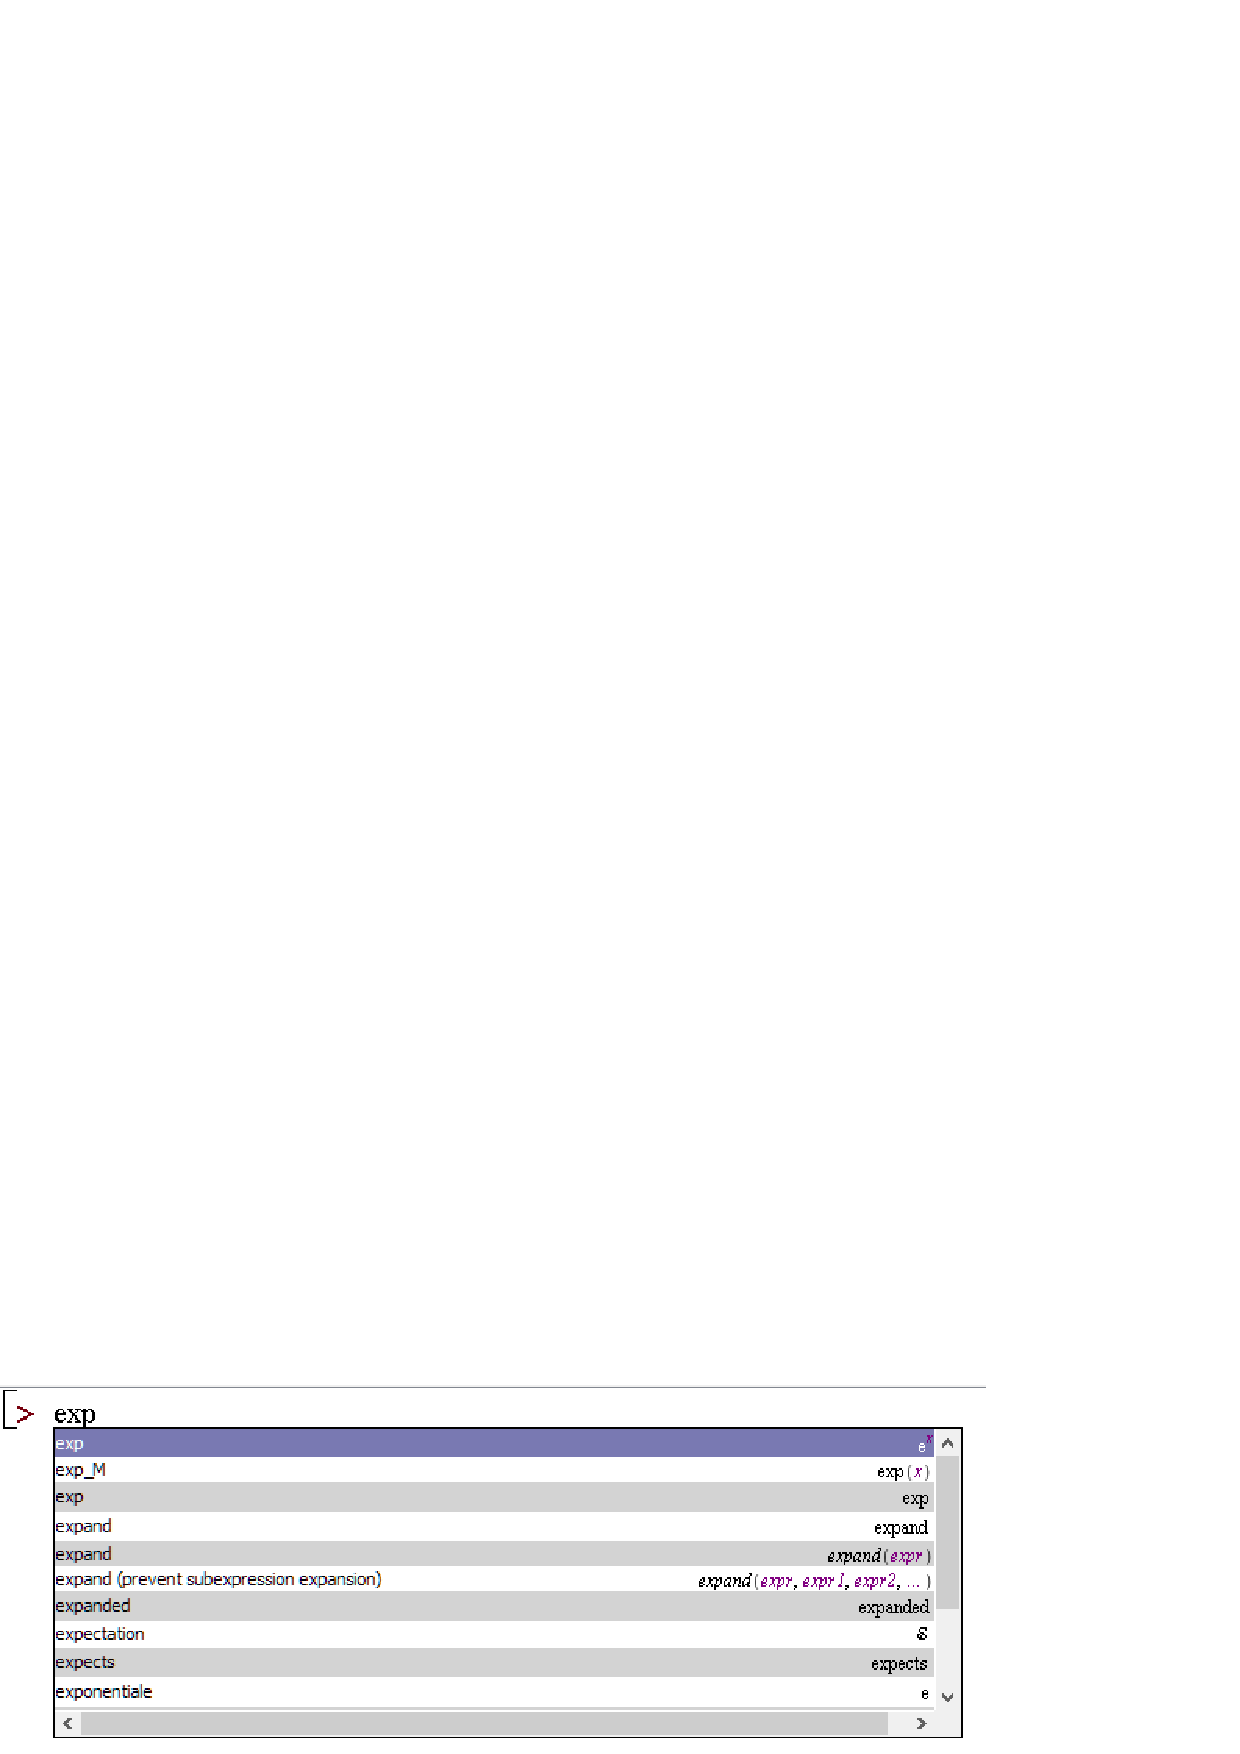
\includegraphics[width=\textwidth]{tutorials/figures/autocomplete.png}
\caption{Using autocomplete with ESC gives a menu of possible commands you are trying to use.}
\end{figure}
From here, you can select the \texttt{exp} command for the exponential function, or possibly the \texttt{expand} command, which we will look at later. If the command requires a parameter, it should already be highlighted so that you can type in its value. If a command has multiple parameters, you can hit the Tab key to highlight the next parameter.

\section{Multiple Commands at Once}

As you may have noticed, each time that we have used Maple input in this tutorial, there is a semicolon \texttt{;} at the end of the line. This used to be required in older versions of Maple, though it is no longer mandatory in modern versions.

\index{mathematical functions!exponential}
\index{mathematical functions!nth root@$n$\textsuperscript{th} root}

The reason why the semicolon continues to be important is because it tells Maple when one command ends and another begins. You can use this to run multiple commands within one Maple input:

\marginnote{Multiple commands can be run at the same time by placing a semicolon \texttt{;} in between them.}
\begin{maplegroup}
\begin{mapleinput}
\mapleinline{active}{1d}{surd(x,3); exp(x);
}{}
\end{mapleinput}
\mapleresult
\begin{maplelatex}
\mapleinline{inert}{2d}{surd(x,3)}{\[\displaystyle \sqrt[3]{x} \]}
\end{maplelatex}
\begin{maplelatex}
\mapleinline{inert}{2d}{exp(x)}{\[\displaystyle {\rm e}^{x} \]}
\end{maplelatex}
\end{maplegroup}
\marginnote{If you use a full colon \texttt{:} instead of a semicolon, then the output of that command is hidden from the screen when it is executed.}

\section{The \% Shortcut}\label{percentage}

\index{ditto operator}

Many of the exercises in the activities will involve executing multiple commands to obtain the answer. Often, this means running a command and then running a second command on the result of the first. Although copying and pasting the result from the first command takes less time than typing it out, it often causes many syntax problems.

Fortunately, Maple provides us with the \% shortcut, also called the ditto operator. Every time a command is run, its output is temporarily stored, much like a scientific calculator will remember what is currently on its screen. Using the \% symbol within another command will use the result of the first command automatically. 

The trouble with this shortcut comes from the fact that you can run Maple input anywhere on the page \textit{in any order}! In the example below, you will only get the correct output if you run the second line \textit{immediately} after running the first line.

\begin{maplegroup}
\begin{mapleinput}
\mapleinline{active}{1d}{x\symbol{94}2 + 5;
}{}
\end{mapleinput}
\mapleresult
\begin{maplelatex}
\mapleinline{inert}{2d}{x^2+5}{\[\displaystyle {x}^{2}+5\]}
\end{maplelatex}
\end{maplegroup}
\index{mathematical functions!square root}
\begin{maplegroup}
\begin{mapleinput}
\mapleinline{active}{1d}{sqrt(%);
}{}
\end{mapleinput}
\mapleresult
\begin{maplelatex}
\mapleinline{inert}{2d}{sqrt(x^2+5)}{\[\displaystyle \sqrt{{x}^{2}+5}\]}
\end{maplelatex}
\end{maplegroup}

To make better use of the \% shotcut, it is the best practice to combine the two consecutive commands on the same Maple input:

\marginnote{The \% shorcut in Maple works much like the \textit{ANS} button on many scientific calculators. The \% will only remember the output of whatever input was run most recently.}

\begin{maplegroup}
\begin{mapleinput}
\mapleinline{active}{1d}{x\symbol{94}2 - 4; sqrt(%);
}{}
\end{mapleinput}
\mapleresult
\begin{maplelatex}
\mapleinline{inert}{2d}{x^2-4}{\[\displaystyle {x}^{2}-4\]}
\end{maplelatex}
\begin{maplelatex}
\mapleinline{inert}{2d}{sqrt(x^2+5)}{\[\displaystyle \sqrt{{x}^{2}+5}\]}
\end{maplelatex}
\end{maplegroup}